\documentclass[11pt]{article}
\usepackage{gset}
\usepackage{preamble}
\begin{document}
	\maintitle{Матан Дз 3}
	1) \textbf{Исследуйте следующие рекуррентные последовательности на сходимость:} \bs
	а) $a_{n + 1} = \sqrt{2a_n}, a_1 = \sqrt{2}$ \bs
	Пусть сущеcтвует $\lim\limits_{n\to \infty} a_n = a \Rightarrow \lim\limits_{n\to \infty} a_{n + 1} = \lim\limits_{n\to \infty} \sqrt{2a_n} \lra a = \sqrt{2a} \lra a = 2$. \bs
	Докажем, что предел существует. \bs
	1) Ограниченность \sspace
	Докажем используя математическую индукцию $0 < a_n \leq 2: P_n$. \sspace
	\textbf{База:} $P_1: 0 < \sqrt{2} \leq 2$ - верно \sspace
	\textbf{Шаг:} $P_{n + 1}: 0 < \sqrt{2a_n} \leq \sqrt{2*2} = 2$ - верно \sspace
	2) Монотонность \sspace
	$a_{n - 1} - a_n = \sqrt{2a_n} - a_n = \sqrt{2a_n} - \sqrt{a_n^2} = \sqrt{a_n}(\sqrt{2} - \sqrt{a_n})$. Так как $0 < a_n \leq 2$, то $\sqrt{a_n}(\sqrt{2} - \sqrt{a_n}) \geq 0$. \sspace
	По теореме Вейерштрасса у последовательности есть предел \bs
	\answer{2}
	\bs 
	b) $a_{n + 1} = \sqrt{6 + a_n}, a_1 = 0$ \bs
	Пусть сущеcтвует $\lim\limits_{n\to \infty} a_n = a \Rightarrow \lim\limits_{n\to \infty} a_{n + 1} = \lim\limits_{n\to \infty} \sqrt{6 + a_n} \lra a = \sqrt{6 + a} \lra a = 3$. \bs
	Докажем, что предел существует. \bs
	1) Ограниченность \sspace
	Докажем используя математическую индукцию $0 \leq a_n \leq : P_n$. \sspace
	\textbf{База:} $P_1: 0 \leq 0 \leq 3$ - верно \sspace
	\textbf{Шаг:} $P_{n + 1}: 0 \leq \sqrt{6 + a_n} \leq \sqrt{6 + 3} = 3$ - верно \sspace
	2) Монотонность \sspace
	$\dfrac{a_{n + 1}}{a_n} = \dfrac{\sqrt{6 + a_n}}{a_n}$ \sspace
	$(\dfrac{\sqrt{6 + a_n}}{a_n})^2 = \dfrac{6 + a_n}{a_n^2} = \dfrac{6}{a_n^2} + \dfrac{1}{a_n} \geq \dfrac{6}{9} + \dfrac{1}{3} = 1 \Rightarrow |\dfrac{a_{n + 1}}{a_n}| \geq 1 \Rightarrow \dfrac{a_{n + 1}}{a_n} \geq 1 $(так как $a_{n} \geq 0$) \sspace - последовательность монотонно возрастает \sspace
	
	По теореме Вейерштрасса у последовательности есть предел \bs
	\answer{3}
	\bs
	c) $a_{n + 1} = \dfrac{2}{3}a_n  + \dfrac{1}{a_n^2}, a_1 = 3$ \bs
	Пусть сущеcтвует $\lim\limits_{n\to \infty} a_n = a \Rightarrow \lim\limits_{n\to \infty} a_{n + 1} = \lim\limits_{n\to \infty}  \dfrac{2}{3}a_n  + \dfrac{1}{a_n^2} \lra a = \dfrac{2a}{3} + \dfrac{1}{a^2}$. \bs
	$ a = \dfrac{2a}{3} + \dfrac{1}{a^2}$ \sspace
	$3a^3 = 2a^3 + 3$ \sspace
	$a = \sqrt[3]{3}$ \bs
	Докажем, что предел существует. \bs
	1) Ограниченность \sspace
	Докажем используя математическую индукцию $\sqrt[3]{3} \leq a_n \leq 3: P_n$. \sspace
	\textbf{База:} $P_1: \sqrt[3]{3} \leq 3 \leq 3: P_n$ - верно \sspace
	\textbf{Шаг:} $P_{n + 1}: $ Докажем используя график функции $f(x) = \dfrac{2x}{3} - \dfrac{1}{x^2}$
	\newpage \quad \sspace
	$f(a_n) = a_{n + 1}$. \\
	Так как $a_n \in [\sqrt[3]{3}; 3]$, то $a_{n + 1} \in [\sqrt[3]{3}; \dfrac{19}{9}] \Rightarrow \sqrt[3]{3} \leq a_{n + 1} \leq 3$
	\[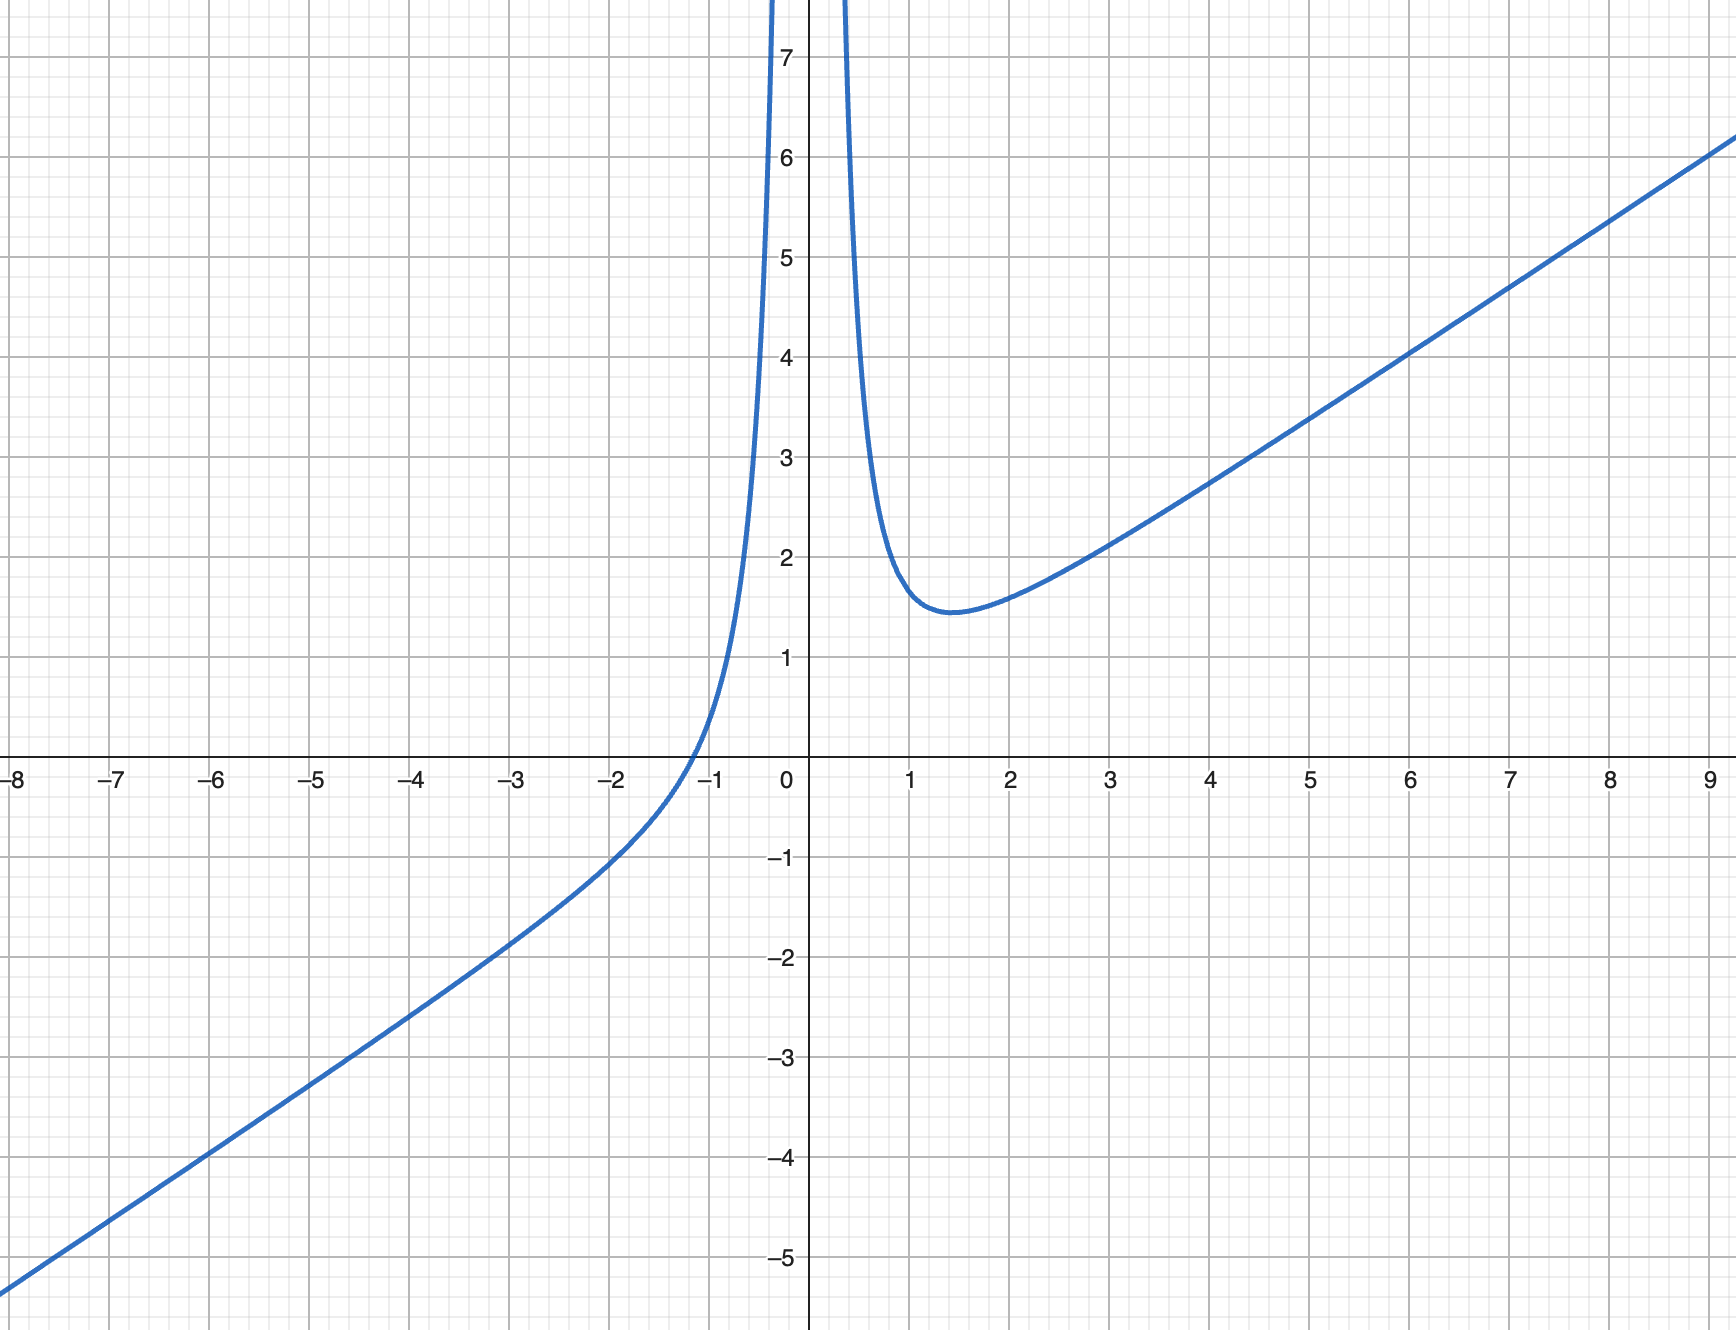
\includegraphics[width=125mm]{img1}\]
	\bs
	\[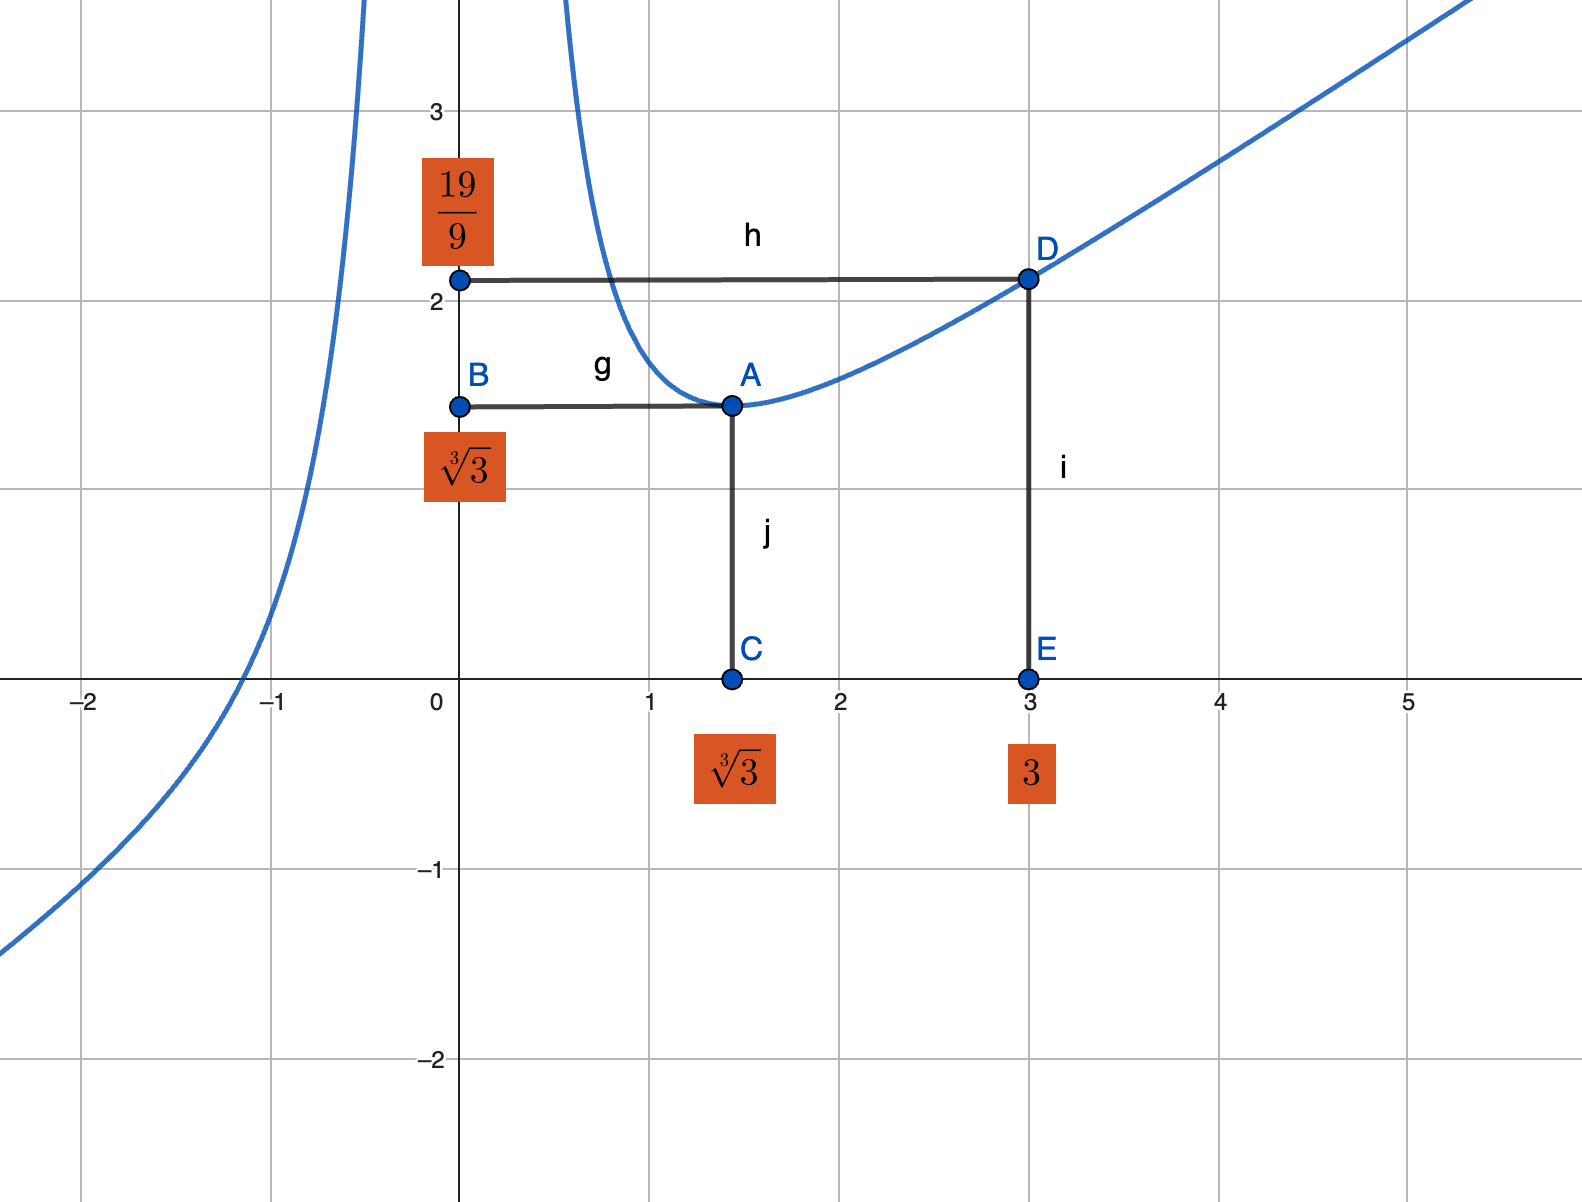
\includegraphics[width=125mm]{img2}\]
	\newpage \quad \sspace
	2) Монотонность \bs
	$a_{n} - a_{n + 1} = \dfrac{a_n}{3} - \dfrac{1}{a_n^2} = \dfrac{a_n^3 - 3}{3a_n^2} \geq 0$. Функция монотонна и ограничена,\\
	\\
	 значит по теореме Вейерштрасса у нее есть предел. \bs
	\answer{$\sqrt[3]{3}$}
	\bs
	d) $a_{n + 1} = 1 + \dfrac{1}{1 + a_n}, a_1 = 1$ \bs
	Пусть существует   $\lim\limits_{n\to \infty} a_n = a \Rightarrow \lim\limits_{n\to \infty} a_{n + 1} = \lim\limits_{n\to \infty} 1 + \frac{1}{1 + a_n} \lra a = 1 + \frac{1}{1 + a} \lra a = \sqrt{2}$ или $a = -\sqrt{2}$ \sspace
	Так как $a_{n + 1} = 1 + \frac{1}{1 + a_n} \geq 1$, то предел $a = -\sqrt{2}$ точно не подходит. Остается доказать существование предела последовательности $a_n$. \bs
	Для этого сначала докажем неравенство $|a_n - a| \leq \lambda|a_{n - 1} - a|, \lambda \in (0; 1) $ \bs
	$|a_n - a| = | 1 + \frac{1}{1 + a_{n - 1}} - 1 - \frac{1}{1 + a}| = | \frac{1 + a - 1 - a_{n - 1}}{(1 + a_{n - 1})(1 + a)}| = \frac{| a - a_{n - 1}|}{(1 + a)(1 + a_{n - 1})} = \lambda|a_{n-1} - a| $  \sspace
	(так как $1 + a \geq 1 \land 1 + a_{n - 1} \geq 1$)
	\bs
	$|a_n - a| = \lambda^n|1 - a| = \lambda^n(\sqrt{2} - 1)$ \bs
	$\lim\limits_{n\to \infty} \bigg\{|a_n - a| = \lambda^n(\sqrt{2} - 1) \bigg\} = 0$ \bs
	Значит по определению a - предел последовательности. 
	\bs
	\answer{$\sqrt{2}$}
	\bs
	2) \textbf{Найти предел:} $\lim\limits_{n\to \infty} \dfrac{a_n}{a_1*a_2\cdots a_{n - 1}}$ \bs
	$a_{n + 1} = a_n^2 - 2, a_1 = 3$ \bs
	Докажем используя  метод математической индукции, что при $n \geq 2$, выполняется: \sspace
	$P_n : a_n^2 - 4 = a_1^2*a_2^2\cdots a_{n - 1}^2 (a_1^2 - 4)$\bs
	\textbf{База:} $P_2: a_2^2 - 4 = a_1^2*(a_1^2 - 4)$ \sspace
	$a_2 = 3^2 - 2 = 7$ \sspace
	$49 - 4 = 9 * (9 - 4)$ - верно \bs
	\textbf{Шаг:} $P_{n + 1}: a_{n + 1}^2 - 4 = a_1^2 * a_2^2 \cdots a_{n}^2(a_1^2 - 4)$ \bs
	$a_{n + 1}^2 - 4 = (a_n^2 - 4)a_n^2$
	\sspace Используя выражение $n + 1$ого члена последовательности: \sspace 
	$(a_n^2 - 2)^2 - 4 = a_n^4 - 4a_n^2$ \space
	$a_n^4 - 4a_n^2 + 4 - 4 = a_n^4 - 4a_n^2$ - верно. \bs
	Далее вычислим предел \bs
	$\lim\limits_{n\to \infty} \dfrac{a_n}{a_1*a_2\cdots a_{n - 1}} = {\lim\limits_{n\to \infty} \sqrt{\dfrac{a_n^2}{a_1^2*a_2^2\cdots a_{n - 1}^2}}} = {\lim\limits_{n\to \infty} \sqrt{\dfrac{ a_1^2*a_2^2\cdots a_{n - 1}^2 (a_1^2 - 4) + 4}{a_1^2*a_2^2\cdots a_{n - 1}^2}}} = \bs = \sqrt{a_1^2 - 4} = \sqrt{9 - 4} = \sqrt{5}$ \bs
	\answer{$\sqrt{5}$}
\end{document}